{}

\section{{Problem 1}}

	\subsection{{Computer Program}}

		\begin{lstlisting}[language=C, caption=\textit{}]
#include <stdio.h>
#include <string.h>
#include <ctype.h>

#define NUM_CHARACTER 1000
#define INDEX_O 0
#define INDEX_1 1

int b = 0, c = 0;

void reverse(char before[], char after[]);

void clean(char before[], char after[]);

void clean(char before[], char after[])
{
    while (before[c] != '\0')
    {
        if (isalnum(before[c]))
        {
            after[b++] = tolower(before[c]);
        }
        c++;
    }
    after[b] = '\0';
}

void reverse (char before[], char after[])
{
    int len = strlen(before);
    if(len == 0)
    {
        after[INDEX_O] = '\0';
    }
    else
    {
        reverse(&before[INDEX_1], after);
        strncat(after, before, INDEX_1);
    }
}

void main(void)
{
    char phrase[NUM_CHARACTER], reversing[NUM_CHARACTER], cleaning[NUM_CHARACTER];
    printf("Please enter a string: ");
    fgets(phrase, NUM_CHARACTER, stdin);
    printf("Original structure of the string: %s", phrase);
    clean(phrase, cleaning);
    printf("Clean structure of the string: %s\n", cleaning);
    reverse(cleaning, reversing);
    printf("Reverse structure of the string: %s\n", reversing);
    if (strcmp(cleaning, reversing) != 0)
    {
        printf("This is not a palindrome.\n");
    }
    else
    {
        printf("This is a palindrome.\n");
    }
}


\end{lstlisting}

	\subsection{{Program Output Screenshot}}

		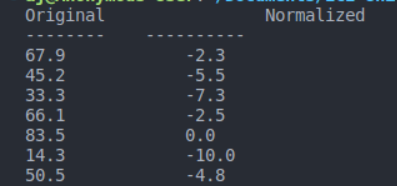
\includegraphics[width=15cm]{problem1.png}
		

		
		
		